%
% Grundlagen Kaptiel
% Zielsetzung: Techniken erklären und zum Projekt hinführen!
%
\chapter{Semantik Web Grundlagen}
\label{cap-grundlagen}
\section{Einführung: Semantic Web und Linked Data} % karl
\label{sec-grundlagen-einf-semweb}
Oft gelesen, selten verstanden. Das \textbf{Semantic Web} ist kein neues Web, es kann wie das Web 2.0 nur als eine Erweiterung aufgefasst werden. Dabei ist diese nur zu einem geringen Teil technischer Natur. Die grundlegenden, technischen Konzepte und Ideen bestehen inzwischen einige Zeit. Auch deren Umsetzung ist in der Informatik-Zeitrechnung fast schon Geschichte. Trotzdem gibt es kaum Anwendungen, die wirklich Gebrauch vom Semantic Web machen. Dies begründet sich vor allem darin, dass es bisher wenige Informationen als so genannte \textbf{Linked Data} (verknüpfte Daten) gibt, was sich jedoch von Tag zu Tag ändert. Weitere Gründe für die verhaltene Entwicklung in der sonst so von Trend und Boom bestimmten IT-Branche ist auch die technische Akzeptanz, z.B. ist RDF nicht direkt intuitiv zu begreifen.


Im Folgenden werden wir von simplen Begriffserklärungen bis hin zu Projekten, die sich den unterschiedlichsten Aufgabenstellungen des Semantic Web widmen, beleuchten.

% Denn hier handelt es sich - wie so oft - um ein klassisches Henne-Ei-Problem\footnote{\url{http://de.wikipedia.org/wiki/Henne-Ei-Problem}}.


\paragraph*{Semantic Web} 
Erweiterung des World Wide Webs. Im Web veröffentlichte Daten sollen durch Standardformate für Maschinen les- und verarbeitbar werden. Ursprung dafür ist der Artikel \cite{Bern01} des Web-Begründers Tim Berners-Lee.
Wikipedia schreibt (\cite{WPSEMWEB}):
\begin{quote}
``Die Informationen im Web sollen von Maschinen interpretiert und automatisch maschinell weiterverarbeitet werden können. Informationen über Orte, Personen und Dinge sollen mit Hilfe des Semantischen Webs von Computern miteinander in Beziehung gesetzt werden können. [...] Bei der Verknüpfung der Informationen in einem Semantischen Web können neue Zusammenhänge entdeckt werden, die zuvor nicht erkennbar waren.''
\end{quote}


\paragraph*{Linked Data} % andreas
\label{linked-data}
Fachbegriff eines bewährten Verfahrens (best practice) zur Beschreibung von Quellen. Das Verfahren definiert die Darstellung, den Zugriff und die Verbindungen der einzelnen Teilstücke von Daten, Informationen und Wissen zu einem großen Ganzen, dem Semantic Web. Das Zusammenfügen erfolgt dabei mittels \gls{URI} und dem \gls{RDF}.

% a term used to describe a recommended best practice for exposing, sharing, and connecting pieces of data, information, and knowledge on the Semantic Web using URIs and RDF." \todo[inline]{Auf deutsch und überarbeiten; Quelle en.wp} 

Die folgende Abbildung \ref{graphic-lod-datasets} zeigt an einem Beispiel, anhand verschiedenster Datenquellen, wie der Zugriff und die Verbindungen erfolgen und wie man dies in einem Graphen darstellen kann.

\newpage
\begin{figure}[htbp]
	\centering
	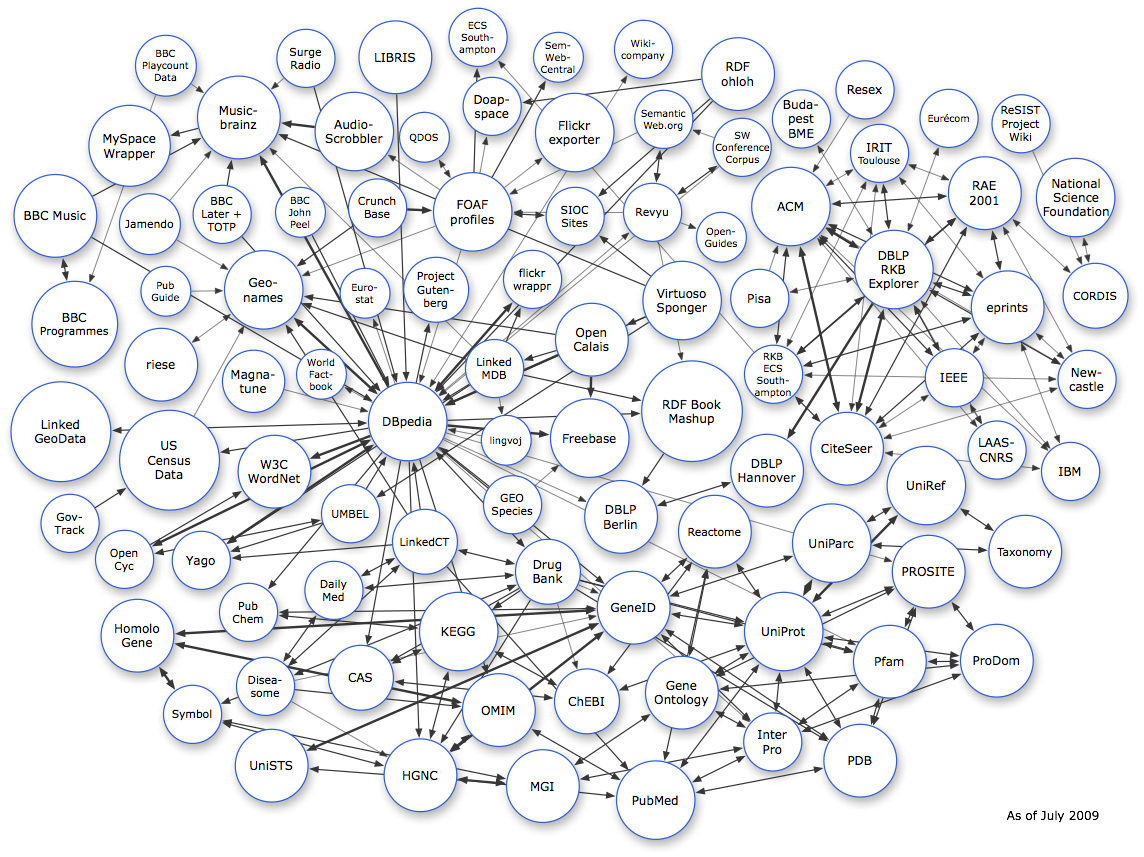
\includegraphics[scale=0.3]{images/lod-datasets_2009-07-14}
	\caption{Linking Open Data: Offene Datenquellen und deren Verbindungen; Quelle: \cite{LINKEDATA}}
	\label{graphic-lod-datasets}
\end{figure}

\section{Triples} % benny 
\label{sec-triples}
Ein Triple besteht im Bezug auf Semantic Web und insbesondere im Bezug auf RDF und OWL aus den drei Elementen Subjekt, Prädikat und Objekt. Die Idee dahinter ist, dass eine Ressource über Subjekte oder Klassen verfügen kann, die bestimmte Eigenschaften haben.
Das Subjekt wird mittels einer \gls{URI} identifiziert. Es kann sich dabei um ein Dokument, einen Gegenstand oder eine Information handeln. Die Eigenschaft, welche eine Ressource hat ist das Prädikat und der Wert dieser Eigenschaft ist das Objekt. Prädikate und Objekte können Zeichenketten sein, aber auch andere Ressourcen. So kann eine rekursive Struktur aufgebaut werden. Ein Triple wird öfters auch Statement genannt.
Eine Möglichkeit Triples darzustellen, zu übertragen oder zu speichern, bietet das N-Triples Format. Dieses zeilenbasierte Format serialisiert das RDF-Format als Klartext. Dieses Format wurde 2004 als offizielle Recommendation vom \gls{W3C} verabschiedet. Turtle ist noch eine Erweiterung von N-Triples, da diese zu wenig Funktionalität bieten. Beispielsweise wurde eine Kurzschreibweise hinzugefügt. Beide Formate sind im wesentlichen Teil des von Tim Berners-Lee vorgeschlagenen Formats N3 (Notation 3), aber beide beschränken sich darauf nur zulässige RDF-Graphen darzustellen. 

\section{RDF}
\gls{RDF} ist ein Framework um Informationen/Metadaten über bestimmte Informationen zu speichern. RDF speichert also sozusagen „Daten über Daten“ (über Daten). Die beschriebenen Informationen sind meist Webressourcen. Dabei spielt es keine Rolle ob die Daten nur einfache Informationen sind oder ein komplexes Objekt. Zum Beispiel können Informationen über den Autor oder das Erstellungsdatum eines Dokuments dargestellt und Informationen über den Inhalt des Dokumentes selber beschrieben werden. Das Hauptziel ist mittels RDF Metadaten automatisch auszuwerten und zu bearbeiten. Weitere Ziele sind das Auffinden von Informationen im Web (Katalogisierung) und Bewertungen von Inhalten (Rating). Außerdem ist RDF ein Baustein des \gls{WOT}, dabei werden über eine Community Webseiten als sicher vermerkt. RDF bietet zusätzlich eine gute Interoperabilität zwischen verschiedenen Metadaten-Systemen.
RDF wird vom W3C bereits seit 1999 entwickelt und ist offen für weitere Erweiterungen.
Das RDF-Framework verwendet die in \ref{sec-triples} Triples um die Informationen zu beschreiben.

\begin{lstlisting}[language=xml,numbers=none,caption=Beispiel für ein einfaches RDF-Dokument,label=code-rdf-grundlage-1]

<?xml version="1.0"?>
<rdf:RDF xmlns:rdf="http://www.w3.org/1999/02/22-rdf-syntax-ns#"
             xmlns:contact="http://www.w3.org/2000/10/swap/pim/contact#">

  <contact:Person rdf:about="http://www.w3.org/People/EM/contact#me">
    <contact:fullName>Eric Miller</contact:fullName>
    <contact:mailbox rdf:resource="mailto:em@w3.org"/>
    <contact:personalTitle>Dr.</contact:personalTitle> 
  </contact:Person>

</rdf:RDF>
\end{lstlisting}
Im Codelisting \ref{code-rdf-grundlage-1} (entnommen aus \cite{RDF-Prim}) findet sich ein kurzes Beispiel für die Beschreibung der Person \flqq Eric Miller\flqq\ in RDF-XML. Darin enthalten sind URIs, welche Ressourcen im Web identifizieren können, Eigenschaften (properties) wie z.B. ``mailbox'' oder ``fullname'' und die Werte der Eigenschaften (values) z.B. ``Eric Miller''. Die XML Elemente werden auch Terms genannt.
Der zugehörige Graph ist in \ref{graphic-rdf-bsp-graph} abgebildet. 
\begin{figure}
	\centering
		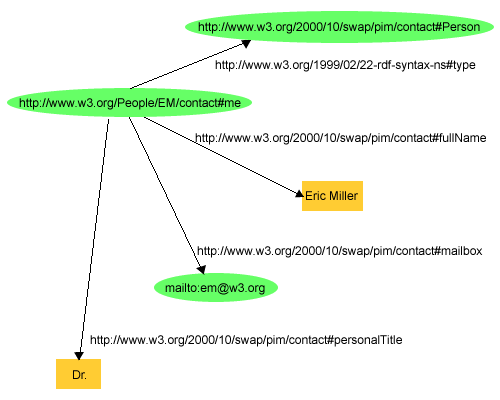
\includegraphics[keepaspectratio,scale=0.6]{images/RDF-bsp}
	\caption{Darstellung des Beispielgraphen}
	\label{graphic-rdf-bsp-graph}
\end{figure}

Durch die Verknüpfung von Daten in Anwendungen werden die Zusammenhänge maschinenlesbar dargestellt. Diese Zusammenhänge können dazu verwendet werden, um dem User weitere Hilfen oder Informationen zu bieten.
\\
Die wichtigsten Eigenschaften von RDF sind:
\begin{itemize}
\item Unabhängigkeit
Jede Domäne kann eigene Prädikate für ihre Subjekte definieren.
\item Austauschbarkeit
Durch die Verwendung von \gls{XML} wird der Austausch und die Kommunikation, zwischen Anwendungen oder Domänen, erheblich vereinfacht.
\item Skalierbarkeit 
Große Mengen von Daten können durch die Einteilung in Triples schnell und effizient verarbeitet werden.
\item Prädikate sind Ressourcen
Durch den rekursiven Aufbau können Prädikate eigene Prädikate haben, welche automatisch weiterverarbeitet werden.
\item Objekte können Ressourcen sein
Wie bei den Prädikaten gilt hier auch der rekursive Aufbau, damit auch diese wieder eigene Ressourcen sein und weiterverarbeitet werden können.
\end{itemize}
Das Ganze hat den Vorteil, dass sich die Daten aus verschieden Anwendungen exportieren lassen, ohne das die Daten der Daten ihre Bedeutungen verlieren.
RDF selbst definiert kein Vokabular für die Beschreibung der Meta Daten, dafür eignet sich beispielsweise \gls{DC}.
Noch zu erwähnen ist, dass RDF nicht durch eine XML DTD definiert ist sondern durch die \gls{EBNF}. Dadurch ist RDF unabhängig von XML.

\paragraph{RDF Syntax}
RDF Dateien können auf zwei verschiedene Arten geschrieben werden, als \frqq Abbreviated\frqq\ oder \frqq Serialization Syntax\frqq. Bei der Serialization werden die Werte als XML-Elemente definiert. In der Abbreviated Syntax werden die Properties als Attribute definiert, dabei ensteht das Problem, dass mache Attribute dann mehrfach in einem XML Element auftauchen.
Nachfolgend werden kurz die wichtigsten Elemente oder Terms beschrieben. Dabei wird nur auf die Abbreviated Syntax eingegangen. 
\newpage
Die Beispiele wurden \cite{W3SRDF} entnommen.
Es gibt fünf wesentliche Kategorien für die XML Notation\cite{XML03}:
\begin{itemize}
\item Das RDF Element \textit{RDF}, welches den Rahmen der Dokuments festlegt. Es ist das Wurzelelement und beinhaltet die verschiedenen Namespaces.
\item \textit{Description} definiert das Subjekt des Triple, dieses wird im \textit{about} Attribut angegeben. Auch sind weitere Informationen, die die Ressource beschreiben enthalten.
\item textit{Container}, welche Eigenschaften zusammenfassen. Die drei vorhandenen Containertypen sind \textit{rdf:Bag}, \textit{rdf:Seq} und \textit{rdf:Alt}. \textit{rdf:Bag} (Tasche, Sack) wird bei ungeordneten Mengen von Aufzählungen verwendet. Bei \textit{rdf:Seq}(für Sequenz) handelt es sich um geordnete Listen, z.B. alphabetisch. \textit{rdf:Alt}(Alternative) wird verwendet, wenn die Aufzählung nur einen vordefinierten Wert annehmen kann. Container können wieder beschrieben werden. Beispielsweise kann der Autor eines \textit{Container} angefügt werden.
\item Der Elementtyp \textit{type} kann auf die Beschreibung eines RDF-Schema verweisen.
\item Anwendungsspezifische Elementtypen zur Beschreibung von Eigenschaften.
\end{itemize}
\begin{lstlisting}[language=xml,numbers=none,caption=Beispiel für die RDF Syntax,label=code-bsp-rdf-syntax]
<?xml version="1.0"?>

<rdf:RDF
xmlns:rdf="http://www.w3.org/1999/02/22-rdf-syntax-ns#"
xmlns:cd="http://www.recshop.fake/cd#">

<rdf:Description
rdf:about="http://www.recshop.fake/cd/Empire Burlesque"
cd:artist="Bob Dylan" cd:country="USA"
cd:company="Columbia" cd:price="10.90"
cd:year="1985" />

</rdf:RDF> 
\end{lstlisting}

In dem oben aufgeführten Codebeispiel wird eine CD von Bob Dylan definiert. Die Elemente \textit{artist}, \textit{country}, \textit{company}, \textit{price} und \textit{year} werden im Namespace \newline \textit{http://www.recshop.fake/cd\#} definiert. Dieser liegt außerhalb von RDF.
\newpage
\begin{lstlisting}[language=xml,numbers=none,caption=Beispiel für geschachtelte Ressourcen in RDF,label=code-bsp-rdf-syntax2]
<?xml version="1.0"?>

<rdf:RDF
xmlns:rdf="http://www.w3.org/1999/02/22-rdf-syntax-ns\#"
xmlns:cd="http://www.recshop.fake/cd\#">

<rdf:Description
rdf:about="http://www.recshop.fake/cd/Empire Burlesque">
  <cd:artist rdf:resource="http://www.recshop.fake/cd/dylan" />
  ...
  ...
</rdf:Description>

</rdf:RDF>
\end{lstlisting}
Im Beispiel \ref{code-bsp-rdf-syntax2} wird gezeigt wie ein geschachtelter Term aufgebaut ist. Dabei hat die \textit{artist} Eigenschaft keinen Wert, sondern eine Referenz auf eine andere Ressource welche weitere Informationen über den Künstler enthält.
\begin{lstlisting}[language=xml,numbers=none,caption=Beispiel für eine Sequenz in RDF,label=code-bsp-rdf-syntax3]
<?xml version="1.0"?>

<rdf:RDF
xmlns:rdf="http://www.w3.org/1999/02/22-rdf-syntax-ns\#"
xmlns:cd="http://www.recshop.fake/cd\#">

<rdf:Description
rdf:about="http://www.recshop.fake/cd/Beatles">
  <cd:artist>
    <rdf:Seq>
      <rdf:li>George</rdf:li>
      <rdf:li>John</rdf:li>
      <rdf:li>Paul</rdf:li>
      <rdf:li>Ringo</rdf:li>
    </rdf:Seq>
  </cd:artist>
</rdf:Description>

</rdf:RDF>
\end{lstlisting}

In \ref{code-bsp-rdf-syntax3} wird eine Sequenz von Werten verwendet. In RDF werden diese Werte von Listen \textit{members} genannt.

Für weitere Informationen über die Syntax und Beispiele können unter \cite{RDF-Prim} oder \cite{W3SRDF} nachgelesen werden.
\paragraph{RDF Schema}
RDF benötigt Erweiterungen um konkret Klassen und Eigenschaften für eine Anwendung nutzen zu können. Für diesen Zweck wurde \gls{RDFS} entwickelt. Mit RDFS kann eine Grammatik definiert werden, um die Inhalte von RDF-Elementen für eine bestimmte Domäne zu modellieren. Es kann also für “kontrolliertes Vokabular” applikationsspezifisch erzeugt und eingesetzt werden. Einfache \gls{Ontologie}n können auf diese Weise formalisiert werden. Der gleiche Gegenstand wird innerhalb einer Applikation oder Ressource immer gleich benannt. Mehr zu Ontologien im Abschnitt über OWL \ref{sec-owl}.
Mit RDFS kann darüber hinaus noch überprüft werden, ob eine Ressource von einem Typ ist, welcher die verwendeten Statements erlaubt oder nicht.
Neben RDFS gibt es noch weitere Ontologien wie \gls{OWL} oder \gls{F-Logic}.

\section{OWL} % benny 
\label{sec-owl}

Die \gls{OWL} ist eine weitere Spezifikation des W3C um Ontologien mit Hilfe formaler Syntax zu erstellen. Bevor nun näher auf OWL eingegangen wird, zuerst noch ein paar Worte zu Ontologien im Allgemeinen.
Eine Ontologie ist die ``Konzeptionalisierung und Kodierung von Expertenwissen mit Hilfe eines strukturierten Glossars und einem vereinbarten Vokabular''\cite{Kred07}. Mit Ontologien werden Informationen und Wissen zusammengefasst und strukturiert, um die Daten austauschbar und maschinenlesbar zu machen. Anschließend können diese Wissensbasen durchsucht, zusammengefügt und editiert werden. Auch können neue Instanzen und Wissensbasen erzeugt werden.
Technisch gesehen basiert OWL auf der RDF-Syntax. Es ist ausdrucksstärker als RDFS und basiert historisch auf \gls{DAML} und \gls{OIL}. OWL stellt drei Untersprachen zur Verfügung, OWL DL, OWL Full und OWL Lite. Die Mächtigkeit der OWL DL (Description Language) ist die Gleiche wie bei der Aussagenlogik (Logik 1. Stufe). Dies bedeutet, dass die Sprache berechen- und entscheidbar ist. OWL Full ist mächtiger als (Logik 2. Stufe) deshalb ist sie nur semi-entscheidbar. Die Lite Version ist ähnlich wie OWL DL, nur dass die Kardinalitäten nur 0 oder 1 sind. 
Mehr zum Thema OWL \cite{OWL096} 

\section{SPARQL} %wiedi
\label{sec-sparql}
\gls{SPARQL}\footnote{\url{http://www.w3.org/2009/sparql/wiki/Main_Page}} (gesprochen ``sparkle'') ist eine Abfragesprache für Graphen.
Der Name ist ein rekursives Akronym für ``SPARQL Protocol and RDF Query Language'' und benennt somit die zwei Bestandteile.
Zum einen beschreibt SPARQL ein Protokoll\footnote{\url{http://www.w3.org/TR/rdf-sparql-protocol/}},
zum anderem aber auch eine Abfragesprache\footnote{\url{http://www.w3.org/TR/rdf-sparql-query/}}.

Die Hauptidee hinter der Abfrage Sprache ist einfaches \gls{Pattern-Matching}.
Ein Untergraph wird mit Platzhaltern beschrieben und wo immer ein Untergraph übereinstimmt wird ein Resultat zurückgegeben.

Anfragen werden an sogenannte SPARQL-Endpoints gestellt, diese verarbeiten die Anfrage und liefern die Resultate zurück.
Die meisten Datenquellen bieten öffentliche SPARQL-Endpoints an über die der Datenbestand abgefragt werden kann.
Der Endpoint von DBPedia (siehe \ref{dbpedia}) ist z.B. unter \url{http://dbpedia.org/sparql} erreichbar.

SPARQL-Endpoints sind \gls{RESTful}\footnote{\url{http://en.wikipedia.org/wiki/Representational_State_Transfer}} Webservices, eine Abfrage ist somit nur ein einfacher HTTP-GET Request.
Im Protokoll-Teil der Spezifikation wird dies genauer beschrieben. 

Die Resultate können, abhängig von der eingesetzten Endpointsoftware, in verschiedenen Formaten zurückgegeben werden.
Die gängigsten Formate sind XML, JSON und Plaintext für ``ASK'' und ``SELECT'' Queries,
sowie RDF/XML, N-Triples, N3 und Turtle für ``DESCRIBE'' und ``CONSTRUCT'' Abfragen.

Um das SPARQL-Protokoll nicht selbst implementieren zu müssen gibt es Bibliotheken für viele Programmiersprachen.
Für JavaScript gibt es sparql.js\footnote{\url{http://www.thefigtrees.net/lee/sw/sparql.js}}, und für Python gibt es SPARQLWrapper\footnote{\url{http://sparql-wrapper.sourceforge.net/}}, welcher einfach anzuwenden ist.
%\todo[inline]{SPARQL beispiele evtl.}
\section{Projekte} % benny 
Verschiedene Projekte befassen sich bereits mit den Aufgaben und Möglichkeiten des Semantic Web. Diese haben teilweise verschiedene Herangehensweisen für die verschiedenen Aufgaben. Teilweise sind diese auch nur Grundlagen für andere Projekte, einige davon werden nun nachfolgend kurz vorgestellt.
\subsection{Suchen}
Die Suchmaschinen, welche die Informationen zusammentragen sind ein wichtiger Bestandteil. In dieser Arbeit werden kurz zwei Beispielsuchmaschinen vorgestellt, welche Ontologien zusammentragen und für Abfragen zugänglich machen.
\subsubsection{Watson} % benny 
Watson ist eine von Knowledge Media Institute entwickelte Suchmaschine zur Auffindung von Ontologien und semantischen Inhalten. Es ist nach eigenen Aussagen das Gateway für das Semantic Web, welches von den Anforderungen des Semantic Web und den Erfahrungen aus früheren Systemen geleitet wird und bildet den Ausgangspunkt für die Auffindung von Ontologien. Aufgaben sind dabei das Sammeln von Daten, deren Analyse und Auswertung, sowie die Beantwortung von Anfragen. Nähere Informationen sind unter \cite{WATSON} zu finden.
\subsubsection{Sindice} % benny 
Sindince ist eine Suchmaschine, welche die über das ganze Web verstreuten Definitionen des Semantic Web sammelt. Dabei spielt es keine Rolle von welcher Art von Seite die Informationen zusammengetragen werden. Verarbeitet werden Daten in den Formaten RDF, RDFa und \gls{Microformats}. Diese zusammengetragenen Informationen können wie bei Watson auch abgefragt werden.
\subsection{Datahubs} % benny 
\label{sec-dathubs}
Datahubs sind Projekte, welche Informationen zusammentragen und in semantischer Form abfragbar machen. Diese Informationen können von Maschinen gelesen und verbunden werden um dem Benutzer Informationen über viele Bereiche hinweg bereitstellen zu können.
\subsubsection{DBpedia} % wiedi + benny
\label{dbpedia}
Die DBPedia ist ein Community Projekt um Wissensinhalte aus Wikipedia zu extrahieren und die Informationen maschinenlesbar im Web zu veröffentlichen.
Interessant ist dabei auch, dass die Daten als Linked-Data auch auf andere Datenquellen verweisen.
Die von Wikipedia eingesetzte Software ``Mediawiki'' kann selbst allerdings noch nicht mit Semantic-Web Daten umgehen. Um dies zu erreichen gibt es das Semantic-Mediawiki\footnote{\url{http://semantic-mediawiki.org}}.
\subsubsection{Freebase} %wiedi
Freebase\footnote{\url{http://www.freebase.com}} ist eine sehr große eigenständige Wissensdatenbank. Daten werden aus vielen verschiedenen Quellen, wie z.B. MusicBrainz\footnote{\url{http://musicbrainz.org}}, Wikipedia und NNDB\footnote{\url{http://www.nndb.com}} als Linked-Data importiert - können jedoch auch von Benutzern wie ein Wiki direkt editiert werden.

